The lunar farside provides a unique accessible environment in that the moon shields it from earth and near-earth radio frequency interference at all times.  Therefore, {\em anything} detected is of scientific interest. Since there is no ionospheric blockage, low frequency observations that are impossible from earth can also be made in an RFI-free environment.  Although the lunar farside will remain an excellent low-RFI site for many years to come, {\em now} is the only time to take completely pristine measurements.  This is an opportunity that will never again present itself.

\subsection{Technosignatures}
Humanity's quest to determine its place in the Universe and whether we are its only inhabitants has driven knowledge and imagination since we first looked to the sky.  Many large telescopes are in consideration in order to help determine if other biological processes are happening in nearby stars (called "biosignatures") and we now also have the capability to explore whether technological signatures exist over a large swath of our Galaxy.  The Breakthrough Listen program has transformed the field and has greatly expanded the search for such technosignatures.  The greatest impediment is the prevalence of radio frequency interference (RFI) made by essentially every device that is electrically powered.

Signals of interest must be carefully sought within this cacophony of RFI.  To differentiate between RFI and a technosignature requires that the technosignature signal is at a frequency/time not inhabited by RFI and the signal must persist and be quite stable over a timeframe of many minutes.  The signals are assumed to be nearly monochromatic and slow-drifting in time.  A series of on-off measurements are used to make sure that the signal-of-interest is coming from the main beam of the telescope and not RFI in a distant sidelobe.  These techniques are incredibly powerful in conducting senstive searches over the available bandwidth, and have the added benefit being able to use very large earth-based telescopes to dramatically increase the sensitivity.  However, many limitations exist on appropriate ranges of frequency and time, and some frequency ranges are so impacted that searches (and radioastronomy generally) are infeasible in those bands.  Signals of short duration (a few seconds) or signals heavily modulated are nearly impossible to discern.  And of course, technosignatures ``behind'' RFI is not detectable (or at least believably so).

\subsection{Transients}
The recent flourishing of the field of radio transients has brought a wealth of information, significantly advancing various areas of physics. Notably, pulsars and fast radio bursts (FRBs) stand out due to their unique potential to reveal new kinds of physics. These astrophysical phenomena offer valuable insights into gravitational waves, cosmology, and plasma physics, among other fields.

\subsubsection{Pulsars}
Pulsars are highly magnetized, rotating neutron stars that emit beams of electromagnetic radiation. They serve as precise cosmic clocks, providing insights into the interstellar medium, gravitational waves, and the fundamental physics of matter under extreme conditions. %Observing pulsars at low frequencies can reveal details about their emission mechanisms and the properties of the intervening space that are not accessible at higher frequencies 

\subsubsection{Fast Radio Bursts}
Fast Radio Bursts (FRBs) are intense, millisecond-duration radio pulses originating from extragalactic sources. Their origins remain one of the most intriguing mysteries in modern astrophysics. %Low-frequency observations of FRBs are crucial for understanding their propagation through the intergalactic medium, potentially unveiling the distribution of baryonic matter and offering clues about the mechanisms driving these bursts 

\subsubsection{Flare Stars}

% This depends if Uranus or Neptune fall in any of the beams throughout the observatories lifetime and what kinda tsys we get at those times. 
% \subsubsection{Solar System Lighting} 

\section{Observation Strategy} % This may be better as a sub-section in the operations section. 

\begin{figure}[h]
    \centering
    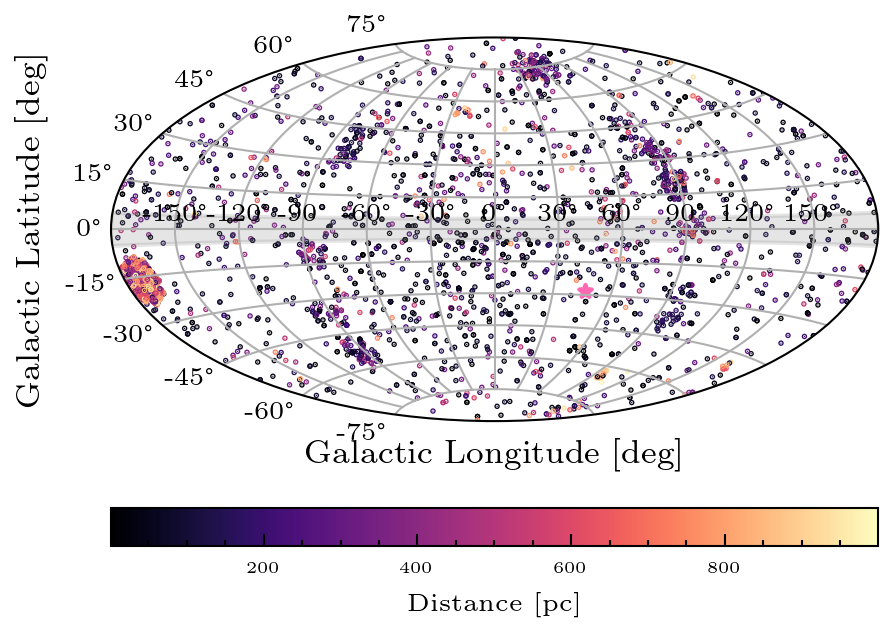
\includegraphics[width=0.6\textwidth]{figures/Science Case Plots/galactic_projection_NEA.png}
    \caption{Some plot here with target of intrests that fall within the zenith pointings and their associated Jy measurements based on Tsys etc. }
    \label{fig:enter-label}
\end{figure}